\newpage
\chapter*{Rozdział 2 \\ \vspace{1cm} Opis zbioru danych i definicje zmiennych}
 \addcontentsline{toc}{chapter}{2. Opis zbioru danych i definicje zmiennych}
 
W pierwszej części rozdziału przedstawiony zostanie sposób zgromadzenia bazy danych, najważniejsze informacje o niej oraz najważniejsze źródła pochodzenia danych. W dalszej części rozdziału szczegółowo opisana zostanie każda zmienna użyta w badaniu, łącznie z jej najważniejszymi statystykami opisowymi. 

\phantomsection				% do hiperlinków dla sekcji w spisie treści
\section*{2.1 Baza danych}
\addcontentsline{toc}{section}{2.1 Baza danych}

Baza danych zawiera 1663 obserwacje 20 zmiennych, z czego tylko 12 najważniejszych zostało użytych w modelowaniu ekonometrycznym. Użyte zostały zmienne, które wydawały się najbardziej istotne w obliczu teorii i mogły dać najciekawsze wnioski badawcze. Sposób doboru filmów do bazy danych był pseudolosowy, o wyborze filmu decydował algorytm napisany przez autora niniejszej pracy. Niestety z powodu braków danych i sposobu ich gromadzenia nie udało się uzyskać czystej losowości. Informacje o filmach zostały sczytane z następujących stron internetowy:

\begin{itemize}
\item http://www.imdb.com/,
\item http://www.filmweb.pl/,
\item http://www.boxofficemojo.com/,
\item http://www.oscars.org/awardsdatabase,
\item http://www.boxoffice.com/,
\item http://www.cinematoria.com/.
\end{itemize}

W związku z tym, iż żadne z powyższych źródeł nie udostępnia swojej bazy danych, informacje o każdym filmie musiały zostać zebrane oddzielnie poprzez sczytanie ich przez program komputerowy z odpowiednich miejsc na stronach internetowych. Co oczywiste otrzymany zbiór danych nie były nigdy wykorzystywany w innych badaniach – został specjalnie zgromadzony na potrzeby modelu. W modelu wykorzystano 1638 obserwacji ze znajdujących się w bazie 1663 ze względu na braki danych niektórych zmiennych.

\phantomsection				% do hiperlinków dla sekcji w spisie treści
\section*{2.2 Charakterystyka zmiennych}
\addcontentsline{toc}{section}{2.2 Charakterystyka zmiennych}
\vspace{0.5cm}

\phantomsection				% do hiperlinków dla sekcji w spisie treści
\subsection*{2.2.1 Zmienna zależna}
\addcontentsline{toc}{subsection}{2.2.1 Zmienna zależna}
\vspace{0.5cm}

\begin{itemize}
	\item[\ding{228}]\textbf{oscar} \\ 
	\\Zmienna binarna, przyjmująca następujące wartości:
  	\begin{itemize}
  	\item[]1 - gdy film lub osoba związana z filmem zdobyła Oscara
  	\item[]0 - w przeciwnym wypadku
  	\end{itemize}
\end{itemize}

\vspace{0.4cm}
{\centering
\textbf{Tabela 1. Charakterystyki zmiennej zależnej oscar.}}
\begin{stlog}

      oscar {\VBAR}      Freq.     Percent        Cum.
\HLI{12}{\PLUS}\HLI{35}
          0 {\VBAR}      1,441       86.65       86.65
          1 {\VBAR}        222       13.35      100.00
\HLI{12}{\PLUS}\HLI{35}
      Total {\VBAR}      1,663      100.00
{\smallskip}

\end{stlog}

\textit{\footnotesize{Źródło: Opracowanie własne.}} \\

Jak widać w bazie przeważają filmy, które nie zdobyły żadnego Oscara, jest ich 1441 czyli blisko 87\% wszystkich obserwacji. Tylko 13\% filmów (222 z 1663) zdobyło choć jedną statuetkę. 

\phantomsection				% do hiperlinków dla sekcji w spisie treści
\subsection*{2.2.2 Zmienne niezależne}
\addcontentsline{toc}{subsection}{2.2.2 Zmienne niezależne}
\vspace{0.5cm}

Zgodnie z tym co zostało napisane we wstępie do niniejszej pracy zmienne niezależne zostały podzielone na 3 główny grupy: zmienne ekonomiczne, zmienne charakteryzujące film i zmienne weryfikujące jakość filmu.
\vspace{0.3cm}
\begin{itemize}
\item \textbf{\large{Zmienne ekonomiczne:}}
\vspace{0.3cm}

Do tej grupy należą zmienne o charakterze ekonomicznym, mierzące koszty wyprodukowania filmu oraz przychody/zyski które dany film wygenerował. Mają one weryfikować wpływ czynników finansowych na prawdopodobieństwo otrzymania Oscara.

  	\begin{itemize}
  	\item[\ding{228}]\textbf{budzet2000} \\
  	\\Ciągła zmienna ilościowa, powstała poprzez przeliczenie budżetów poszczególnych filmów na dolary w cenach stałych z 2000 roku. \\
  	
\vspace{3cm}
	
{\centering
\textbf{Tabela 2. Charakterystyki zmiennej budzet2000.}}
\begin{stlog}	
	
    Variable {\VBAR}       Obs        Mean    Std. Dev.       Min        Max
\HLI{13}{\PLUS}\HLI{56}
  budzet2000 {\VBAR}      1644    4.19e+07    3.72e+07   12389.04   2.48e+08
{\smallskip}
	
\end{stlog}

\textit{\footnotesize{Źródło: Opracowanie własne.}} \\
  	
Zmienna budzet2000 przyjmuje wartości w przedziale od około 12 tysięcy do 248 milionów dolarów, ze średnią na poziomie 42 milionów.\\

\begin{figure}[h]
\begin{centering}
  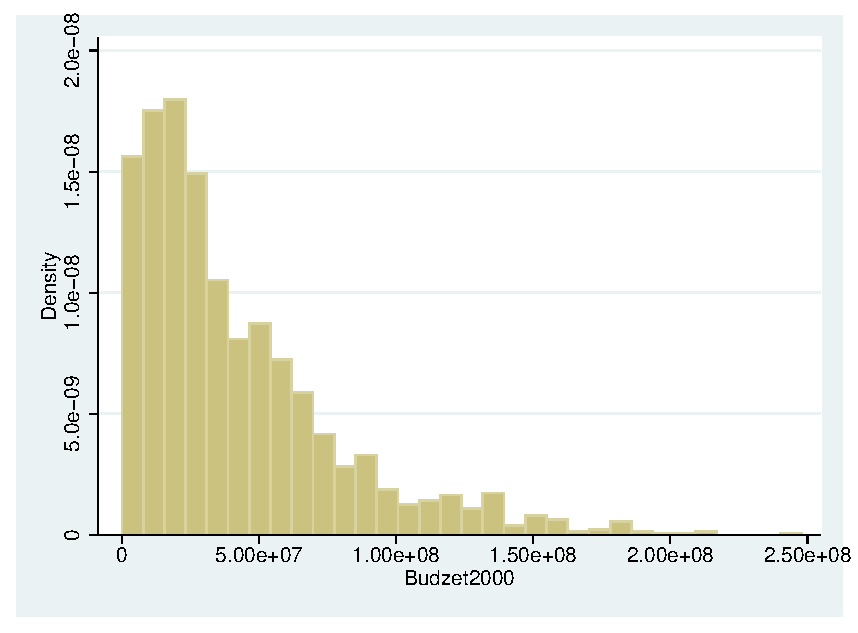
\includegraphics[height=3in]{Rysunki//budzet2000}
    \caption{\textbf{Histogram zmiennej budzet2000.}}
\end{centering}
\end{figure}

\textit{\footnotesize{Źródło: Opracowanie własne.}} \\
  	
  	\item[\ding{228}]\textbf{przychody2000} \\
  	\\Ciągła zmienna ilościowa, powstała poprzez przeliczenie przychodów  poszczególnych filmów z kas biletowych na dolary w cenach stałych z 2000 roku. Można by przypuszczać, iż na wartość tej zmiennej może wpływać wartość zmiennej zależnej, czyli fakt zdobycia Oscara może implikować wyższe przychody filmu. Jednak ze względu na termin gali oskarowej - koniec lutego, najmłodszy film który może wygrać statuetkę może mieć dwa miesiące, czyli jest już u schyłku swojej kinowej popularności. Fakt ten sprawia, iż wpływ zdobycia Oscara na przychody z kas jest marginalny, co potwierdzają badania E. Helmera przedstawione w artykule \textit{The Value of an Oscar} \cite{helmer13}.\\
 
\vspace{3cm}
	
{\centering
\textbf{Tabela 3. Charakterystyki zmiennej przychody2000.}}
\begin{stlog}	
	
    Variable {\VBAR}       Obs        Mean    Std. Dev.       Min        Max
\HLI{13}{\PLUS}\HLI{56}
przycho{\tytilde}2000 {\VBAR}      1657    1.61e+08    2.41e+08   23714.63   4.61e+09
{\smallskip}

	
\end{stlog}

\textit{\footnotesize{Źródło: Opracowanie własne.}} \\

Średnia wartość zmiennej przychody2000 wynosi około 161 mln dolarów, minimum tej zmiennej wyniosło około 24 tysiące, a maksimum 4,6 miliarda dolarów.

\vspace{0.5cm}

\begin{figure}[h]
\begin{centering}
  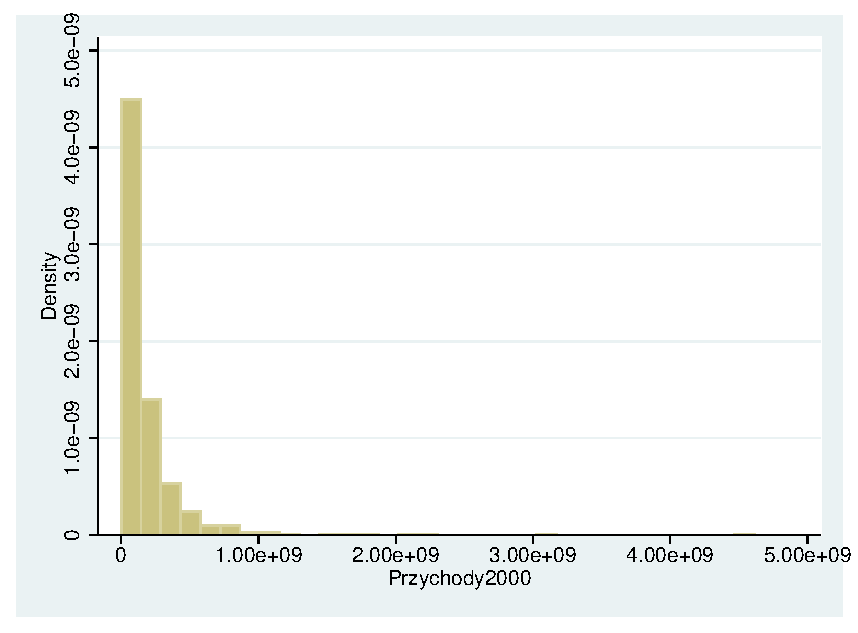
\includegraphics[height=3in]{Rysunki//przychody2000}
    \caption{\textbf{Histogram zmiennej przychody2000.}}
\end{centering}
\end{figure}

\textit{\footnotesize{Źródło: Opracowanie własne.}} \\
 	 
  	\item[\ding{228}]\textbf{roi}\\
  	\\Ciągła zmienna ilościowa, jest to wskaźnik zwrotu z inwestycji w film (w \%), wyliczony według wzoru:
  	
  	\begin{equation}
	roi=\frac{przychody2000-budzet2000}{budzet2000}*100
	\end{equation}
	
\vspace{0.5cm}
	
{\centering
\textbf{Tabela 4. Charakterystyki zmiennej roi.}}
\begin{stlog}	
	
    Variable {\VBAR}       Obs        Mean    Std. Dev.       Min        Max
\HLI{13}{\PLUS}\HLI{56}
         roi {\VBAR}      1638    1615.718    33486.27  -99.54134    1288939
{\smallskip}

\end{stlog}

\textit{\footnotesize{Źródło: Opracowanie własne.}} \\


Zmienna roi przyjmuje wartości od -99.54\% do blisko 1288939\%, przy średniej 1616\%.
  	
  	\end{itemize}

\vspace{0.5cm}
\item \textbf{\large{Zmienne charakteryzujące film:}}
\vspace{0.3cm}

	Jest to grupa zmiennych, która przedstawia najważniejsze cechy filmu takie jak gatunek, czas trwania czy miejsce wyprodukowania. Są to czynniki niewątpliwie bezpośrednio lub pośrednio brane pod uwagę przez członków Amerykańskiej Akademii Sztuki i Wiedzy Filmowej, gdy decydują się oni na głosowanie na konkretny film.

	\begin{itemize}
  	\item[\ding{228}]\textbf{gatunek} \\
  	\\Dyskretna zmienna jakościowa przedstawiająca wiodący gatunek filmu. Przyjmuje ona następujące poziomy:
  	\begin{itemize}
  	\item[0] - Dramat
  	\item[1] - Komedia
  	\item[2] - Film animowany
  	\item[3] - Film akcji
  	\item[4] - Fantasy
  	\item[5] - Sci-Fi
  	\item[6] - Sensacyjny
  	\item[7] - Thriller
  	\item[8] - Horror
  	\item[9] - Inny gatunek
  	\end{itemize}
  	
 \vspace{0.5cm}
	
{\centering
\textbf{Tabela 5. Charakterystyki zmiennej gatunek.}}
\begin{stlog}	
	
  gatunek10 {\VBAR}      Freq.     Percent        Cum.
\HLI{12}{\PLUS}\HLI{35}
     Dramat {\VBAR}        624       37.52       37.52
    Komedia {\VBAR}        383       23.03       60.55
  Animowany {\VBAR}         85        5.11       65.66
      Akcja {\VBAR}         63        3.79       69.45
    Fantasy {\VBAR}         74        4.45       73.90
     Sci-Fi {\VBAR}        118        7.10       81.00
 Sensacyjny {\VBAR}         82        4.93       85.93
   Thriller {\VBAR}         98        5.89       91.82
     Horror {\VBAR}         95        5.71       97.53
       Inny {\VBAR}         41        2.47      100.00
\HLI{12}{\PLUS}\HLI{35}
      Total {\VBAR}      1,663      100.00
{\smallskip}

\end{stlog}

\textit{\footnotesize{Źródło: Opracowanie własne.}} \\

Rozkład poszczególnych gatunków w próbce wydaje się dobrze reprezentować strukturę współczesnej kinematografii.
Pierwszy poziom zmiennej (dla dramatu) został przyjęty jako poziom bazowy i nie wprowadzony do modelu, pozostałe zmienne zostały rozkodowane do binarnych postaci: _Igatunek_1,_Igatunek_2, _Igatunek_3, _Igatunek_4, _Igatunek_5, _Igatunek_6, _Igatunek_7, _Igatunek_8, _Igatunek_9, gdzie 1 oznacza, że film należy do danego gatunku, a 0 że nie należy.

\vspace{2cm}

	\item[\ding{228}]\textbf{ekranizacja} \\
	\\Binarna zmienna jakościowa wskazująca czy film jest ekranizacją powieści, artykułu, biografii lub sztuki teatralnej. Zmienna przyjmuje następujące poziomy:
	\begin{itemize}
	
	\item[1] - gdy film jest ekranizacją
	\item[0] - w przeciwnym wypadku
	
	\end{itemize}
	
	 \vspace{0.5cm}
	
{\centering
\textbf{Tabela 6. Charakterystyki zmiennej ekranizacja.}}
\begin{stlog}	

 Ekraniacja {\VBAR}      Freq.     Percent        Cum.
\HLI{12}{\PLUS}\HLI{35}
          0 {\VBAR}      1,216       73.12       73.12
          1 {\VBAR}        447       26.88      100.00
\HLI{12}{\PLUS}\HLI{35}
      Total {\VBAR}      1,663      100.00
{\smallskip}

\end{stlog}

\textit{\footnotesize{Źródło: Opracowanie własne.}} \\
	
	Ponad jedna czwarta filmów w próbce (26,88\%) jest ekranizacją. 
	
	\vspace{0.3cm}
	
	\item[\ding{228}]\textbf{kraj_prod} \\
	\\Zmienna kraj_prod jest zmienną binarną, jakościową, reprezentującą pochodzenie filmu na zasadzie:
	\begin{itemize}
	
	\item[1] - gdy film jest produkcją wyłącznie amerykańską
	\item[0] - gdy film jest produkcją spoza Stanów Zjednoczonych, lub z udziałem Stanów jednoczonych i innych krajów
	
	\end{itemize}
	Taki podział pochodzenia filmów został przyjęty ze względu fakt, iż w Stanach Zjednoczonych od zarania kinematografii tworzyło się najwięcej filmów. 
	
		 \vspace{0.5cm}
	
{\centering
\textbf{Tabela 7. Charakterystyki zmiennej kraj_prod.}}
\begin{stlog}	

kraj_produk {\VBAR}
        cji {\VBAR}      Freq.     Percent        Cum.
\HLI{12}{\PLUS}\HLI{35}
          0 {\VBAR}        735       44.20       44.20
          1 {\VBAR}        928       55.80      100.00
\HLI{12}{\PLUS}\HLI{35}
      Total {\VBAR}      1,663      100.00
{\smallskip}

\end{stlog}

\textit{\footnotesize{Źródło: Opracowanie własne.}} \\

	Tabel 7 przedstawia, iż podział filmów w próbce na wyłącznie amerykańskie i inne jest prawie równomierny, nieznacznie przeważają te pierwsze, jest ich 928, czyli prawie 56\%.
	
\vspace{0.3cm}	
	
	\item[\ding{228}]\textbf{milosc} \\
	\\Binarna zmienna jakościowa wskazująca czy w filmie pojawia się wątek miłosny, czy też nie. Przyjmuje ona następujące poziomy: 
	\begin{itemize}
	
	\item[1] - gdy osią filmu jest wątek miłosny
	\item[0] - w przeciwnym razie	
	
	\end{itemize}
	
	 \vspace{0.5cm}
	
{\centering
\textbf{Tabela 8. Charakterystyki zmiennej milosc.}}
\begin{stlog}	

	     Milosc {\VBAR}      Freq.     Percent        Cum.
\HLI{12}{\PLUS}\HLI{35}
          0 {\VBAR}      1,531       92.06       92.06
          1 {\VBAR}        132        7.94      100.00
\HLI{12}{\PLUS}\HLI{35}
      Total {\VBAR}      1,663      100.00
{\smallskip}

\end{stlog}

\textit{\footnotesize{Źródło: Opracowanie własne.}} \\

Jak widać tylko w 132 filmach spośród 1663 osią filmu jest wątek miłosny, stanowi to zaledwie 8\% wszystkich filmów w próbce.

\vspace{0.3cm}	
	
	\item[\ding{228}]\textbf{czas_trwania} \\
	\\Quasi-ciągła zmienna ilościowa reprezentująca czas trwania filmu w minutach. 
	
		 \vspace{1cm}
	
{\centering
\textbf{Tabela 9. Charakterystyki zmiennej czas_trwania.}}
\begin{stlog}	

    Variable {\VBAR}       Obs        Mean    Std. Dev.       Min        Max
\HLI{13}{\PLUS}\HLI{56}
czas_trwania {\VBAR}      1663    112.9357    21.73786         70        230
{\smallskip}

\end{stlog}

\textit{\footnotesize{Źródło: Opracowanie własne.}} \\

Średni czas trwania filmu wynosi blisko 113 minut, najkrótszy film trwa 70 minut, a najdłuższy 230, czyli blisko 4 godziny. 
	
\begin{figure}[h]
\begin{centering}
  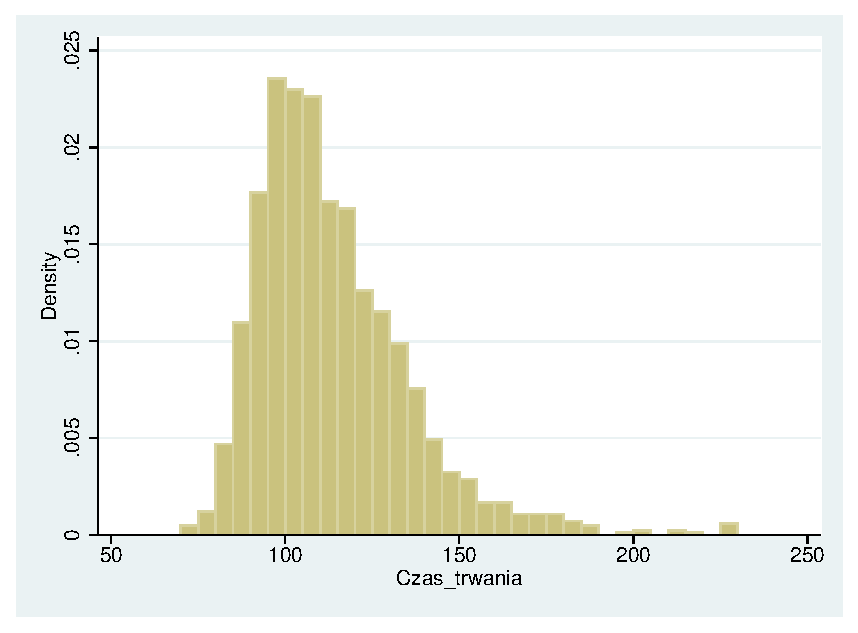
\includegraphics[height=3in]{Rysunki//czastrwania}
    \caption{\textbf{Histogram zmiennej czas_trwania.}}
\end{centering}
\end{figure}

\textit{\footnotesize{Źródło: Opracowanie własne.}} \\

\end{itemize}

	\vspace{0.5cm}
	\item \textbf{\large{Zmienne weryfikujące jakość filmu:}}
	\vspace{0.3cm}
	
Grupa zmiennych reprezentująca uznanie jakie dany film uzyskał w środowisku filmowym, mierzone w liczbie nagród na festiwalach i liczbie nominacji do Oscara. Literatura wskazuje, iż zmienne z tej grupy najbardziej znacząco wpływają na prawdopodobieństwo zdobycia Oscara.
	
	\begin{itemize}
	\vspace{0.5cm}
	\item[\ding{228}]\textbf{nominacje} \\
	\\Zmienna ilościowa przyjmująca wartości ze zbioru liczb naturalnych, reprezentująca liczbę nominacji do Oscara jaką dany film uzyskał.
	
\vspace{0.5cm}
	{\centering
\textbf{Tabela 10. Charakterystyki zmiennej nominacje.}}
\begin{stlog}	

  Nominacje {\VBAR}      Freq.     Percent        Cum.
\HLI{12}{\PLUS}\HLI{35}
          0 {\VBAR}      1,126       67.71       67.71
          1 {\VBAR}        206       12.39       80.10
          2 {\VBAR}         77        4.63       84.73
          3 {\VBAR}         51        3.07       87.79
          4 {\VBAR}         47        2.83       90.62
          5 {\VBAR}         29        1.74       92.36
          6 {\VBAR}         20        1.20       93.57
          7 {\VBAR}         29        1.74       95.31
          8 {\VBAR}         26        1.56       96.87
          9 {\VBAR}         15        0.90       97.78
         10 {\VBAR}         14        0.84       98.62
         11 {\VBAR}         11        0.66       99.28
         12 {\VBAR}          6        0.36       99.64
         13 {\VBAR}          5        0.30       99.94
         15 {\VBAR}          1        0.06      100.00
\HLI{12}{\PLUS}\HLI{35}
      Total {\VBAR}      1,663      100.00
{\smallskip}

\end{stlog}

\textit{\footnotesize{Źródło: Opracowanie własne.}} \\

Jak można odczytać z tabli 10 tylko około 32\% filmów w bazie uzyskało nominacje do statuetki, z czego większość, bo 12 punktów procentowych uzyskało tylko jedną nominacje. Pod tym względem próbka użyta w badaniu nie jest reprezentatywna, gdyż nominacje do Oscara może uzyskać rocznie maksymalnie 120 filmów/osób związanych z filmami (24 kategorie, 5 nominacji w kategorii), co stanowi promil rocznej światowej produkcji, szczególnie w ostatnich latach gdy przemysł filmowych zaczął się bujnie rozwijać w Indiach i Nigerii. Maksymalna liczba nominacji uzyskanych przez jeden film wynosi 15.
	
\vspace{0.5cm}	
	\item[\ding{228}]\textbf{zlote_globy} \\
	\\Zmienna ilościowa przyjmująca wartości ze zbioru liczb naturalnych, reprezentująca liczbę Złotych Globów jaką dany film uzyskał.
	
	\vspace{3cm}
	{\centering
\textbf{Tabela 11. Charakterystyki zmiennej zlote_globy.}}
\begin{stlog}	

Zlote_globy {\VBAR}      Freq.     Percent        Cum.
\HLI{12}{\PLUS}\HLI{35}
          0 {\VBAR}      1,489       89.54       89.54
          1 {\VBAR}        101        6.07       95.61
          2 {\VBAR}         32        1.92       97.53
          3 {\VBAR}         22        1.32       98.86
          4 {\VBAR}         12        0.72       99.58
          5 {\VBAR}          4        0.24       99.82
          6 {\VBAR}          3        0.18      100.00
\HLI{12}{\PLUS}\HLI{35}
      Total {\VBAR}      1,663      100.00
{\smallskip}

\end{stlog}

\textit{\footnotesize{Źródło: Opracowanie własne.}} \\

Tylko 174 spośród 1663 filmów znajdujących się w bazie danych uzyskało co najmniej jednego Złotego Globa, z czego większość (101) uzyskała tylko jedną tego typu nagrodę. Maksymalna liczba statuetek zdobytych przez jeden film wynosi 6.
	
\vspace{0.5cm}
\item[\ding{228}]\textbf{bafta} \\
	\\Zmienna ilościowa przyjmująca wartości ze zbioru liczb naturalnych, reprezentująca liczbę nagród Brytyjskiej Akademii Sztuk Filmowych i Telewizyjnych (BAFTA) jaką dany film uzyskał.
	
	\vspace{0.5cm}
{\centering
\textbf{Tabela 12. Charakterystyki zmiennej bafta.}}
\begin{stlog}	

      BAFTA {\VBAR}      Freq.     Percent        Cum.
\HLI{12}{\PLUS}\HLI{35}
          0 {\VBAR}      1,461       87.85       87.85
          1 {\VBAR}        100        6.01       93.87
          2 {\VBAR}         50        3.01       96.87
          3 {\VBAR}         24        1.44       98.32
          4 {\VBAR}         11        0.66       98.98
          5 {\VBAR}          7        0.42       99.40
          6 {\VBAR}          7        0.42       99.82
          7 {\VBAR}          3        0.18      100.00
\HLI{12}{\PLUS}\HLI{35}
      Total {\VBAR}      1,663      100.00
{\smallskip}

\end{stlog}

\textit{\footnotesize{Źródło: Opracowanie własne.}} \\	

Podobnie jak w przypadku Złotych Globów, większość filmów w próbce nie zdobyło nagrody BAFTA (87,85\%), z tych które zdobyły ponad połowa otrzymała tylko jedną statuetkę. Maksymalna liczba wyróżnień jakie dany film uzyskał wyniosła 7.
	
	\end{itemize}

\end{itemize}

